%
\documentclass[reprint,amsmath,amssymb,aps,floatfix, prl]{revtex4-1}
%
\usepackage{verbatim}
\usepackage{graphicx}
\usepackage{caption}
\usepackage{dcolumn}
\usepackage{bm}
\usepackage{float}
\usepackage{wrapfig}
\usepackage{placeins}
\usepackage{ifthen}
\usepackage{xr}
%
\externaldocument[supp-]{supplement}
%
\begin{document}
%
\title{Weird scaling for 2-D avalanches: \\Curing the faceting, and scaling in the lower critical dimension}
%
\author{L. X. Hayden}
\affiliation{ LASSP, Physics Department, Cornell University \\
 Ithaca, NY 14853-2501, United States}
 \author {Archishman Raju}
 \affiliation {The Rockefeller University, New York, NY 10065}
 \author{James P. Sethna}
 \affiliation{LASSP, Physics Department, Cornell University \\
 Ithaca, NY 14853-2501, United States}
%
\date{\today}
%
\begin{abstract}
The non-equilibrium random-field Ising model is well studied, yet there are outstanding questions. In two dimensions, power law scaling approaches fail and the critical disorder is difficult to pin down. Additionally, the presence of faceting on the square lattice creates avalanches that are lattice dependent at small scales. We propose two methods which we find solve these issues. First, we perform large scale simulations on a Voronoi lattice to mitigate the effects of faceting. Secondly, the invariant arguments of the universal scaling functions necessary to perform scaling collapses can be directly determined using our recent normal form theory of the Renormalization Group. This method has proven useful in cleanly capturing the complex behavior which occurs in both the lower and upper critical dimensions of systems and here captures the 2D NE-RFIM behavior well. The obtained scaling collapses span over a range of a factor of ten in the disorder and a factor of $10^4$ in avalanche cutoff. They are consistent with a critical disorder at zero and with a lower critical dimension for the model equal to two. 
\end{abstract}
%
\maketitle

The non-equilibrium random-field Ising model (NE-RFIM) is a model of long-standing interest. This model, albeit simple, contains the necessary ingredients to describe hysteretic and avalanche behaviors in a diverse set of systems. Barkhausen noise in magnets~\cite{Bertotti98} decision making in socio-economics~\cite{Bouchaud13}, absorption and desorption in superfluids~\cite{Lilly96, Detcheverry04} as well as the effects of nematicity in high $T_c$ superconductors~\cite{Bonetti04, Carlson06, Phillabaum2012} can each be understood in terms of `crackling noise' naturally described by the NE-RFIM. \par
%
Although the NE-RFIM itself has been around in various forms since the 1970s~\cite{ImryMa75}, there are still a number of open questions:
%
\begin{itemize}
	\item Is it in the same universality class as the equilibrium model?
	\item Is the lower critical dimension two?
	\item What is the value of the critical disorder?
	\item Is power law scaling sufficient to capture the behavior?
\end{itemize}
%
It has long been debated whether the equilibrium and non-equilibrium versions of the model are in the same universality class. This question of universality has been approached in a number of ways which have suggested the same class for the two models~\cite{Maritan94, Perez-Reche04, Colaiori04, LiuDahmen09, LiuDahmen09-2,BalogTissierTarjus14}. Recently, however, evidence has been provided that this is not the case~\cite{BalogTarjusTissier18}. Our findings pretty clearly imply this latter result. \par
%
Another open question concerns the lower critical dimension (LCD) of the non-equilibrium model. For the equilibrium case, the LCD is accepted to be two~\cite{BrayMoore85} and there is evidence to believe the same is true of the front-propagation model~\cite{Drossel98}. For the nucleated model, there have been conflicting analysis including work suggesting that the LCD is two~\cite{Perkovic95,Perkovic96}, that power-laws are indeed able to capture the behavior and no crossover occurs in 2D~\cite{Spasojevic11, Spasojevic11-2}, and even that a lower critical dimension does not exist for this model~\cite{Thongjaomayum13,Kurbah15,Shukla16,Shukla17}. Here, we find the success of our results to be consistent with a LCD of two. \par
%
Yet another open question is what value $r_c$ takes in two dimensions for the nucleated model. In the nucleated model, the critical disorder appears to decrease with dimension, going from $5.96 \pm 0.02$ in 5D to $2.16 \pm 0.03$ in 3D~\cite{Sethna06}. This behavior in conjunction with the observation that for both the equilibrium and front-propagation problems, $r_c$ is found to be zero~\cite{Drossel98} suggests that $r_c$ may be quite small. The results we present here are consistent with $r_c=0$.\par
%
Finally, it has yet to be resolved whether a power law form is sufficient to describe the behavior in 2D.  Fitting assuming a power law form, Vives {\em et al.} found $r_c$ to take the value $0.75 \pm 0.03$~\cite{Vives95}. More recently, on a much larger square lattice, Spasojevic {\em et al.} find $r_c=0.54\pm0.02$~\cite{Spasojevic11, Spasojevic11-2} collapsing over a range of $r \in [0.64, 0.70]$. We expect this discrepancy to be replicated in simulations on a larger scale with $r_c$ taking a yet smaller value and suggest this type of inconsistency in power law scaling points to a deficit in its ability to accurately capture the critical behavior in 2D.\par
%
Power law scaling collapses have long been a preferred method for demonstrating that the behavior of a critical system is well understood. That this type of heuristic procedure can work so well in such a widespread number of applications is initially surprising and leads naturally to the question of when and why this approach fails. For example, in the two-dimensional non-equilibrium random-field Ising model (2D NE-RFIM),  attempted collapses assuming power law scaling perform in very limited ranges of disorder~\cite{Spasojevic11, Spasojevic11-2, Perkovic96, KuntzPhD}, which we argue is a symptom of non-power law scaling. This failure can also be observed in a number of other systems, particularly at their lower and upper critical dimension. Recently, Raju et. al.~\cite{Raju17} have been successful in describing the non-linearities that arise in renormalization group flows from the perspective of normal form theory. This fomulation provides a systematic method to perform scaling collapses. In the cases for which power laws work well, the dynamics can be described simply by the presence of a hyperbolic fixed point; the eigenvalues are non-zero and there is no qualitative change in the stability of the fixed points. We propose it is the presence of a transcritical bifurcation in the disorder flow equation that corresponds to the rise in complexity needed to describe simulation data of the 2D NE-RFIM. By considering the form the flow equations should take, we are able to provide concrete non-linear scaling variables which enable collapse of our data over a range of a factor of ten in the disorder.\par
%
In addition to the application of our normal form theory of the Renomalization Group, another key component to the success of our collapses is an approach to dealing with the faceting. Running simulations on a square lattice leads to distortions in the shape of the distributions of interest due to lattice effects as the critical point is approached. Long, unnaturally straight avalanche boundaries for small disorder arise which serve to effectively decrease the simulation size. To combat this, we run our simulations on a Voronoi lattice~\cite{RFIM2Dsupp}.  Although this could in principle introduce an amount of intrinsic disorder, we find the Voronoi lattice to be effective in combating faceting effects, enabling clean collapses over a range of a factor of ten in the disorder, a significantly larger range than the current available collapses which use data in a range $\approx 10\%$.\par
%
The model considered is an avalanche model with nearest neighbor coupling $J$ and a randomized bias $r$ under the influence of an adiabatically increasing field $h$. Avalanche size is denoted $s$. Following the convention of Bray and Moore~\cite{BrayMoore85} for the equilibrium model, we define a parameter $w$ which corresponds to the ratio of the disorder $r$ over the coupling $J$ and determine its RG flow equation through symmetry considerations. In principle, there are an infinite series of terms. Using only analytic changes of variables, however, it is possible to remove all terms of $O(4)$ or higher without removing any universal behavior ~\cite{RFIM2Dsupp}. The final form of the flow equation for $w$ is given by 
%
\begin{equation}
	\label{eq:TruncNF}
	\frac{dw}{d\ell}=w^2+B w^3 ,
\end{equation}
\noindent which corresponds to the normal form of a transcritical bifurcation~\footnote{The traditional transcritical bifurcation normal form~\cite{Strogatz14} $dw/d\ell = w^2$ is derived using the implicit function theorem, but involves changes of variables that alter critical properties in singular ways. Eq.~\ref{eq:TruncNF} is the simplest form that can be reached by successive polynomial changes of variables.}. We may directly solve for the correlation length $\xi\sim(1/w + B)^{-B}\exp(1/w)$ in the normal form variables ~\cite{RFIM2Dsupp}.\par
%
Next consider the flow equations for $s$ and $h$. The eigenvalues for these are given by $\lambda_s=d_f$ and $\lambda_h$ respectively where $d_f$ denotes the fractal dimension. In each case, the zero eigenvalue of $w$ gives rise to cross terms between $s$ and $w$ and $h$ and $w$. Again, in principle, we have an infinite number of possible terms but most all terms may be removed with a polynomial change of variables.   The flow equations for $s$ and $h$ are hence given by
%
\begin{equation}
	\begin{split}
		&\frac{ds}{d\ell}= -d_f s-C s w ,\\ 
		&\frac{dh}{d\ell}= \lambda_h h+F h w
	\end{split}
\end{equation}
%
\noindent where in higher dimensions $d_f = 1/\sigma \nu$ and $\lambda_h = \beta \delta / \nu$. In two dimensions, the individual exponents $\sigma \to 0$ and
$\nu$ and $\beta \delta \to \infty$, keeping the combinations we use finite.  The coefficients $B$, $C$, and $F$ are \underline{universal}. Just as the linear terms at ordinary (hyperbolic) fixed points yield universal critical exponents, these terms control universal dependences of physical behavior with changes in the control parameters. Note that, while they cannot be set to zero by a coordinate change, they may have universal values equal to zero, especially in special cases like the lower critical dimension.\par
%
The appropriate scaling variables to collapse the data can be directly calculated from the flow equations~\cite{RFIM2Dsupp}. The invariant scaling combination obtained takes the form $s/\Sigma(w)$ where $\Sigma(w)$ is a nonlinear function of $w$. We allow for an undetermined scale factor $\Sigma_s$. The resulting form is given by 
%
\begin{equation}
 	\label{eq:SigmaOfw}
	\Sigma(w) = \Sigma_s \bigg{(}B+\frac{1}{w}\bigg{)}^{-B d_f+C}\exp \bigg{(}\frac{d_f}{w}\bigg{)} .
\end{equation}
%
\noindent Likewise for $h$, we obtain:
%
\begin{equation}
 	\label{eq:etaOfw}
	\eta(w) = \eta_s\bigg{(}B+\frac{1}{w}\bigg{)}^{B \lambda_h-F}\exp \bigg{(}-\frac{\lambda_h}{w}\bigg{)}
\end{equation}
%
\noindent where $(h-h_{max})/\eta(w)$ is invariant under the RG, and $\eta_s$ is another scale factor. \par
%
First consider the area weighted size distribution $A(s|w)$. In analogy with three dimensions, we take $A(s|w) = s^{-1}v_s^x \mathcal{A}(v_s^y)$ where $v_s$ is the scaling variable and the prefactor of $s^{-1}$ arises from normalization constraints with $v_s=s/\Sigma(w)$ from Equation~\ref{eq:SigmaOfw}. The avalanche size distribution also depends on an unknown universal scaling function, $\mathcal{A}$. To perform scaling collapses via a fit, we assume a form for this equation~\cite{RFIM2Dsupp}. The associated collapse is shown in Figure \ref{fig:As_collapse}. \par
%
Likewise, in analogy with three dimensions, we obtain $dM/dh(h|w)=\eta(w)^{-1} d\mathcal{M}/dh(v_h)$ where $v_h=(h-h_{max})/\eta(w)$ is the scaling variable~\cite{RFIM2Dsupp}. The associated collapse is shown in Figure \ref{fig:dMdh_collapse}.
%
\begin{figure}
	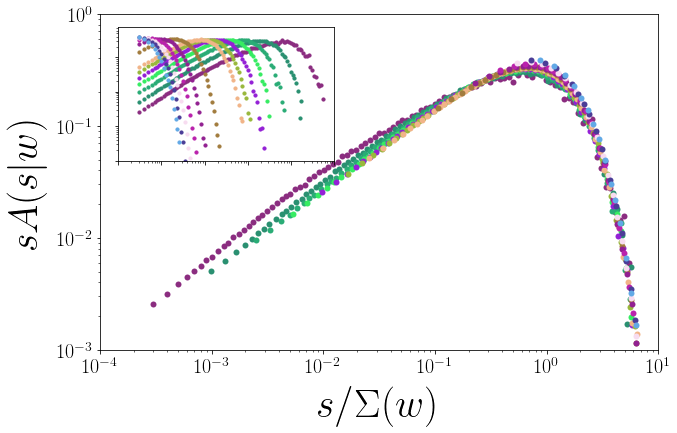
\includegraphics[scale=0.3]{A_collapse_inset.png}
  	\caption{Scaling collapse of the area weighted avalanche size distribution $A(s|w)$ for $w$ ranging from $0.8$ to $8.0$. There is a slight bulge at $s/\Sigma(w)\sim10^{-2}$ for small $w$.}
  	\label{fig:As_collapse}
\end{figure}
%
\begin{figure}
	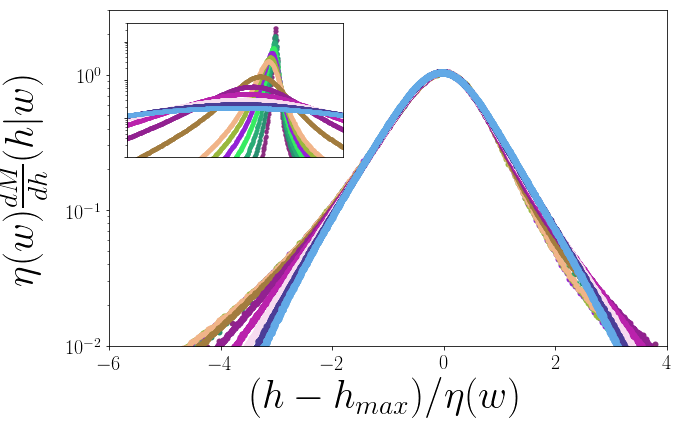
\includegraphics[scale=0.3]{dMdh_collapse_inset.png}
  	\caption{ Scaling collapse of the change in magnetization of the sample with respect to the field $\frac{dM}{dh}(h|w)$ for values of $w$ ranging from $0.8$ to $8.0$. }
  	\label{fig:dMdh_collapse}
\end{figure}
%
Through performing the scaling collapses we are provided with values of $\Sigma$ and $\eta$ for each value of disorder, $r$.  Using the nonlinear scaling forms for each of these we may then extract values for the associated parameters. An unconstrained fit yields a fractal dimension larger than two, the dimension of the system, which is unphysical. The 2D avalanches we consider appear compact. This suggests that the fractal dimension should be given by $d_f=2$ and that the maximum avalanche size should scale as the square of the correlation length. For this reason, we expect also that $\Sigma(w)\sim\xi^2$ and set $C=0$. Imposing these constraints, the fits obtained are able to describe the data well, as shown in Figure~\ref{fig:comparison}.\par
%
We expect the statistical errors and dependence on functional forms chosen for the universal scaling functions to be small. It is useful, however, to consider finite size effects at small $r$ and lattice effects for large $r$.  To compute these error bars,  we performed the collapses and subsequent fits of the nonlinear forms using subsets of the disorders for which we have data [11 out of 13 points]. The errors given are the standard deviation of the values determined in this way. The best fit values with associated errors are given in Table~\ref{tab:params}. Likewise, the standard deviation for both $\Sigma$ and $\eta$ are provided for points in the overlap of the subsets. The error bars for $\Sigma$ and $\eta$ are smaller than the datapoints (Figure~\ref{fig:comparison}). \par
%
Note that the best fit value of $r_c$ is found to be less than zero. There are several possible explanations for this. One, $r_c<0$ could indicate the Voronoi lattice used introduces an amount of intrinsic disorder. This is certainly plausible as random bond and random field disorder are expected to belong to the same universality class~\cite{Dahmen96, Vives95}. Alternatively, constraining $r_c=0$ we obtain a comparable fit by including an alternative normal form, $NF_{\textrm{alt}}$, differing from $\Sigma(w)$ and by analytic corrections to scaling (expected for the larger disorders considered)~\cite{RFIM2Dsupp}. In either case, the results are consistent with $r_c=0.$ \par
%
\begin{table*}
	\centering
	\begin{tabular}{|c|c|c|c|c|c|}
	\hline
	& $NF$ & $NF_0$ & $NF_{\textrm{alt}}$ & $NF_{\textrm{Harris}}$ & Conjecture\\
	\hline
	$r_c$ & $-0.46 \pm 0.06$ & \textbf{0} &  \textbf{0} & $-0.46\pm0.06$ & $[-0.5,0.0]$\\
	$\lambda_h$ & $0.52 \pm 0.07$ & $0.24\pm0.08$ & $0.70\pm0.05$ & \textbf{1} & $1$\\
	$B$ & $-0.15 \pm 0.01$ & $0.039\pm0.007$ & $-0.76\pm0.14$ & $-0.25\pm0.03$ & $[-0.8, 0.0]$\\
	$F$ & $1.33 \pm 0.12$ & $2.02\pm0.13$ & $0.45\pm0.04$ & $0.45\pm0.06$ & $[0.0,0.5]$\\
	$C$ & \textbf{0} & $1.76\pm0.28$ &  \textbf{0} & \textbf{0} & 0\\
	$d_f$ & \textbf{2} & \textbf{2} & \textbf{2} & \textbf{2} & 2\\
	\hline
	\end{tabular}
		\caption{Table of the parameter values determined through a joint fit of $\Sigma(w)$ and $\eta(w)$. $NF$ corresponds to the transcritical form and $NF_{\textrm{alt}F}$ to the alternative transcritical form described in~\cite{RFIM2Dsupp}. $NF_0$ corresponds to the transcritical form with $r_c=0$ and $NF_{\textrm{Harris}}$ to $\lambda_h=1$, the Harris criteria. To compute the error bars,  we performed the collapses and subsequent fits of the nonlinear forms using subsets of the disorders for which we have data [11 out of 13 points]. The errors given are the standard deviation of the values determined in this way. Values in bold were fixed in the corresponding fit. }
	\label{tab:params}
\end{table*}
%
As a test of our finding that the 2D NE-RFIM corresponds to a transcitical bifurcation, we may compare the fits obtained to those using different underlying assumptions. In particular, it is straightforward to calculate $\Sigma$ and $\eta$ assuming a hyperbolic fixed point (corresponding to power law scaling) and a pitchfork bifurcation~\cite{RFIM2Dsupp}. For each of these cases we can perform a fit to the values of $\Sigma(w)$ and $\eta(w)$ extracted from the collapse. The comparison of these fits are shown in Figure~\ref{fig:comparison}.\par
%
\begin{figure}
		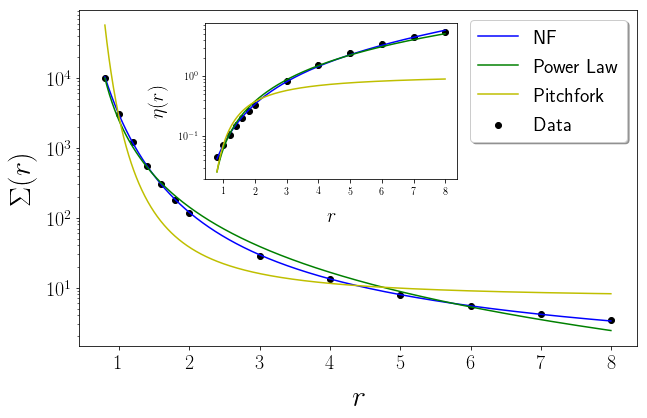
\includegraphics[width=0.5\textwidth]{comparison.png}
		\caption{ Comparison of the best fit of $\Sigma(w)$ and $\eta(w)$ derived with different functional forms of $\frac{dw}{dl}$. We have $w=(r-r_c)/s_s$ such that $\Sigma(r)=\Sigma(w)$ and $\eta(r)=\eta(w)$. `NF' corresponds to $\Sigma$ and $\eta$ derived from the transcritical normal form, `Power Law' the hyperbolic (power law) form and `Pitchfork' the pitchfork form.}
		\label{fig:comparison}
\end{figure}
%
It is particulary illuminating to consider the behavior of $1/\log\Sigma(w)$. For a transcritical bifurcation, the exponential divergence (ignoring $B$ and $C$ in Equation~\ref{eq:SigmaOfw}) gives
%
\begin{equation}
	\frac{1}{\log\Sigma(w)} \sim \frac{1}{d_f} w .
\end{equation}
%
\noindent Hence, if the behavior corresponds to a transcritical bifurcation, we would expect a plot of $1/\log\Sigma$ to scale linearly with the disorder. A comparison of the linear fit to $1/\log\Sigma$, along with the plots of $1/\log\Sigma$ for the best fits with a power law and pitchfork form are shown in Figure~\ref{fig:logplot}.
%
\begin{figure}
		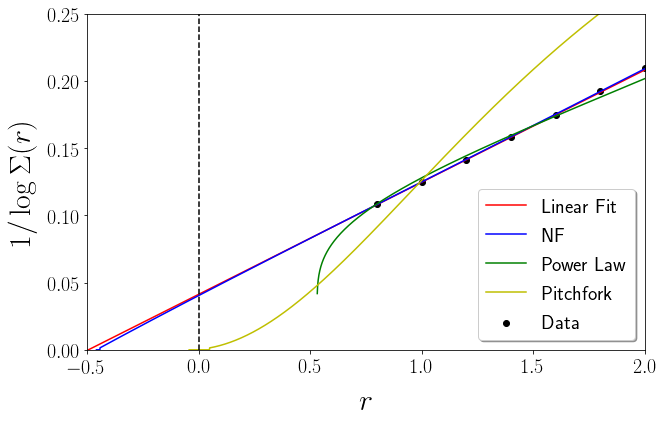
\includegraphics[width=0.5\textwidth]{logplot.png}
		\caption{Comparison of $1/\log\Sigma(w)$ for the best fit of $\Sigma(w)$ derived with different functional forms of $\frac{dw}{dl}$. We have $w=(r-r_c)/s_s$ such that $\Sigma(r)=\Sigma(w)$. `NF' corresponds to $\Sigma$ derived from the transcritical normal form, `Power Law' the hyperbolic (power law) form and `Pitchfork' the pitchfork form.}
		\label{fig:logplot}
\end{figure}
%
\noindent The results clearly support a transcritical bifurcation, with $r_c<0$, and challenge the alternative power law and pitchfork assumptions.\par
%
Simulation data of the 2D non-equilibrium random-field Ising model on a lattice which suppresses faceting is explained well by the presence of a transcritical bifurcation, and is incompatible with power law scaling or pitchfork normal forms without large corrections to scaling. This provides evidence that (1) the universality class of the equilibrium and non-equilibrium models are indeed different and that (2) power law scaling (which is governed by a hyperbolic fixed point) is not the correct approach for this system in this regime. The latter conclusion, in turn, is consistent with (3) the LCD of the model being equal to two, or perhaps close to two.   \par
%
Although the transcitical bifurcation provides the best description of our simulation data, the corresponding parameter values are difficult to pin down. There are a number of restrictions we can make to the parameter values and still obtain a reasonable joint fit of $\Sigma(w)$ and $\eta(w)$ For example, we may require that the Harris criteria saturates, that $r_c=0$~\cite{Perkovic96} or that the coefficient of the quintic order term $B=0$. Each of these provides a good description of our data and are discussed in~\cite{RFIM2Dsupp}. \par
%
In three and higher dimensions~\cite{Perkovic96,Kuntz00}, measuring a
variety of avalanche properties was crucial in pinning down the
universal critical exponents and scaling functions. $dM/dH$ Fand the
cumulative avalanche size distribution, measured here, were supplemented by
measurements of finite-size scaling, avalanche correlation functions,
avalanche sizes binned in $H$, spanning avalanches, avalanche durations,
and average avalanche temporal shapes. Larger system sizes should be possible
with improved Voronoi data structures; Fig.~\ref{fig:logplot} implies that
whether $r_c=0$ or is negative would be definitively answered by a simulation
big enough to contain avalanches with $1/\log(\Sigma) = 0.05$, so with
$L \sim \sqrt(\Sigma) = e^{10} \approx 22,000$.\par
%
In summation, performing large scale simulations on a Voronoi lattice and analyzing the RG flow equations yields valuable insight into the behavior of the NE-RFIM in 2D. The obtained scaling collapses span over a range of a factor of ten in the disorder and a factor of $10^4$ in avalanche cutoff. They are consistent with a critical disorder at zero and with a lower critical dimension for the model equal to two. \par
%
This work was partially supported by NSF grants  DMR-1719490 and DGE-1144153. AR acknowledges support from the Simons Foundation. We thank A. Alan Middleton, Gilles Tarjus, and Karin A. Dahmen for helpful discussions. 

\bibliography{RFIM2D}{}

\end{document}
